\begin{center} \resizebox{0.98\textwidth}{!}{ 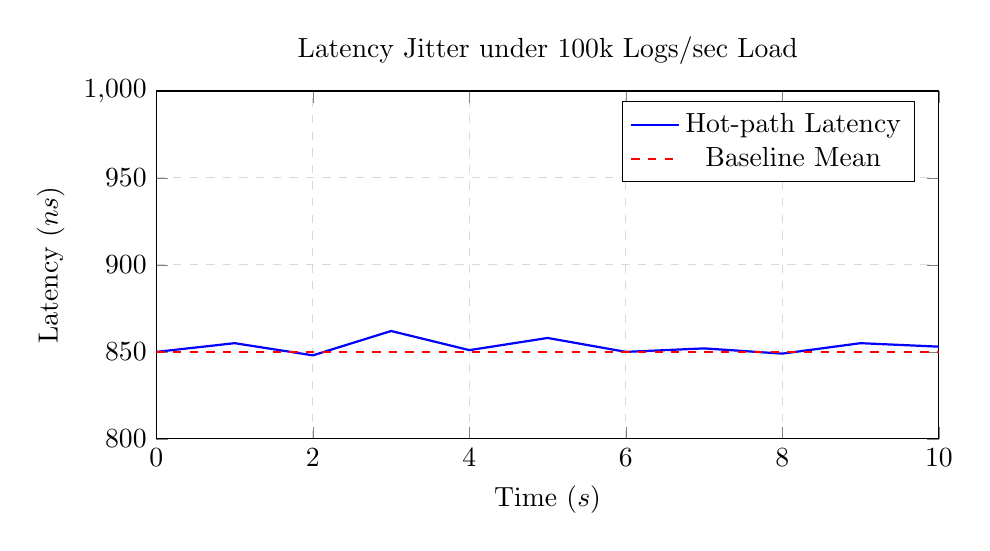
\begin{tikzpicture} \begin{axis}[ width=0.95\columnwidth, height=6cm, xlabel={Time ($s$)}, ylabel={Latency ($ns$)}, xmin=0, xmax=10, ymin=800, ymax=1000, xtick={0,2,4,6,8,10}, ytick={800,850,900,950,1000}, grid=both, grid style={dashed, gray!30}, legend pos=north east, title={Latency Jitter under 100k Logs/sec Load} ] \addplot[color=blue, thick, mark=none] coordinates { (0,850) (1,855) (2,848) (3,862) (4,851) (5,858) (6,850) (7,852) (8,849) (9,855) (10,853) }; \addlegendentry{Hot-path Latency} \addplot[color=red, dashed, thick] coordinates {(0,850) (10,850)}; \addlegendentry{Baseline Mean} \end{axis} \end{tikzpicture} } \end{center}